% coding:utf-8

% Ausführen in R: 
% Sweave("C:/Daten/Daniel/studium/git_repo/sem2/stoc/sw10/sw10_6.Rnw",encoding='UTF-8')

\section{Aufgabe 6}
\begin{Schunk}
\begin{Sinput}
> d.nebel <- read.table("sw10_6.dat",header=T,sep=",")
> nebel.v=d.nebel[,2]
> nebel.dist=d.nebel[,3]
\end{Sinput}
\end{Schunk}

\subsection{a}
\begin{Schunk}
\begin{Sinput}
> plot(nebel.v,nebel.dist)
\end{Sinput}
\end{Schunk}
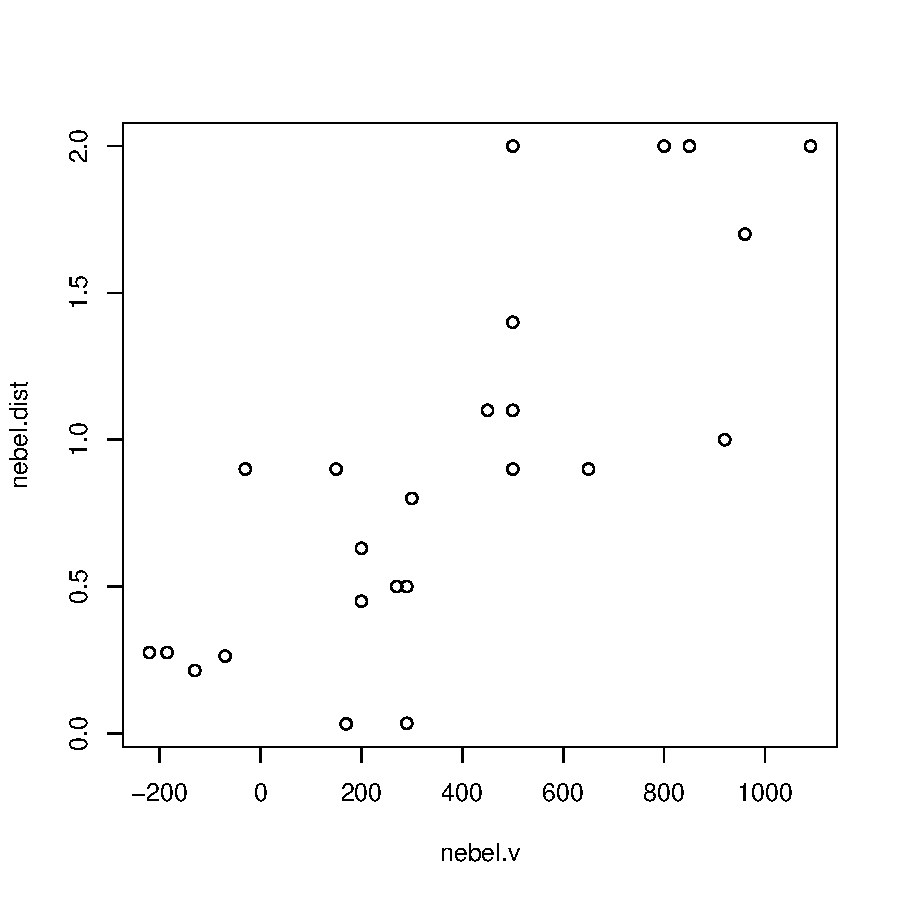
\includegraphics{sw10_6-002}

\subsection{b}
\begin{Schunk}
\begin{Sinput}
> lm(nebel.dist ~ nebel.v)
\end{Sinput}
\begin{Soutput}
Call:
lm(formula = nebel.dist ~ nebel.v)

Coefficients:
(Intercept)      nebel.v  
   0.399098     0.001373  
\end{Soutput}
\begin{Sinput}
> plot(nebel.v,nebel.dist)
> abline(lm(nebel.dist ~ nebel.v))
\end{Sinput}
\end{Schunk}
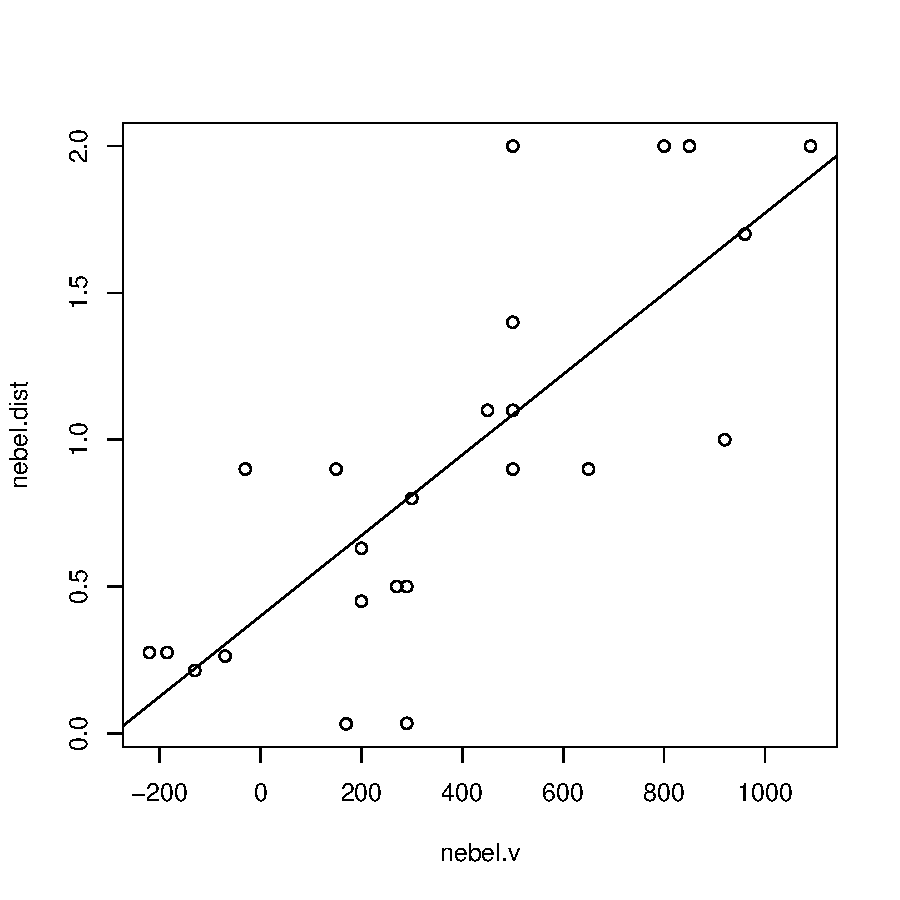
\includegraphics{sw10_6-003}
